\documentclass{acmsiggraph}                     % final
%\documentclass[annualconference]{acmsiggraph}  % final (annual conference)
%\documentclass[review]{acmsiggraph}            % review
%\documentclass[widereview]{acmsiggraph}        % wide-spaced review
%\documentclass[preprint]{acmsiggraph}          % preprint

%% Uncomment one of the five lines above depending on where your paper is
%% in the conference process. ``review'' and ``widereview'' are for review
%% submission, ``preprint'' is for pre-publication, and ``final'' is for
%% the version to be printed. The ``final'' variant will accept the 
%% ``annualconference'' parameter, which changes the height of the space
%% left clear for the ACM copyright information.

%% The 'helvet' and 'times' packages define the typefaces used for
%% serif and sans serif type in this document. Computer Modern Roman 
%% is used for mathematics typesetting. The scale factor is set to .92
%% to bring the sans-serif type in line with the serif type.


\usepackage{hyperref}

\usepackage[scaled=.92]{helvet}
\usepackage{times}
\usepackage[brazil]{babel}
\usepackage[latin1]{inputenc}


%\usepackage{multicol}
\usepackage{url}
\usepackage{wrapfig}
\usepackage[portugues,boxed]{algorithm2e}


%% The 'graphicx' package allows for the inclusion of EPS figures.

\usepackage{graphicx}

%% use this for zero \parindent and non-zero \parskip, intelligently.

\usepackage{parskip}

%% Optional: the 'caption' package provides a nicer-looking replacement
%% for the standard caption environment. With 'labelfont=bf,'textfont=it',
%% caption labels are bold and caption text is italic.

\usepackage[labelfont=bf,textfont=it]{caption}

%% If you are submitting a paper to the annual conference, please replace 
%% the value ``0'' below with the numeric value of your OnlineID. 
%% If you are not submitting this paper to the annual conference, 
%% you may safely leave it at ``0'' -- it will not be included in the output.

\onlineid{0}

%% Paper title.

\title{Vistas Explodidas: um estudo sobre o trabalho \emph{Automated generation of interactive 3D exploded view diagrams}}

%% Author and Affiliation (single author).

%%\author{Roy G. Biv\thanks{e-mail: roy.g.biv@aol.com}\\Allied Widgets Research}

%% Author and Affiliation (multiple authors).

\author{F�bio Markus Miranda\thanks{e-mail: fmiranda@inf.puc-rio.br}\\PUC-Rio}

%% Keywords that describe your work.

\keywords{exploded view, visualization}

%%%%%% START OF THE PAPER %%%%%%

\begin{document}

%\teaser{
%  \includegraphics[width=1.5in]{sample.png}
%  \caption{Lookit! Lookit!}
%}

%% The ``\maketitle'' command must be the first command after the
%% ``\begin{document}'' command. It prepares and prints the title block.

\maketitle

%% Abstract section.

\begin{abstract}
Este trabalho implementa a proposta descrita em \emph{Automated generation of interactive 3D exploded view diagrams} para a visualiza��o de modelos 3D complexos com a utiliza��o da t�cnica de vista explodida. Com ela, � poss�vel ter uma vis�o global do modelo e entender a rela��o entre as diversas partes que o comp�e, sem perda de nenhum detalhe, como ocorre em outras t�cnicas.

A base do trabalho � a gera��o de um \emph{grafo de explos�o} que ir� ditar como as diferentes partes que comp�e um modelo 3D se relacionam, qual a dire��o de explos�o de cada uma e em qual ordem se dar� a explos�o. Uma discuss�o � feita ao final do trabalho, mostrando diferentes modelos de teste explodidos.
\end{abstract}

%% ACM Computing Review (CR) categories. 
%% See <http://www.acm.org/class/1998/> for details.
%% The ``\CRcat'' command takes four arguments.

%\CRcatlist{
%  \CRcat{I.3.5}{Computer Graphics}
%  {Computational Geometry \& Object Modeling}{};
%  \CRcat{I.3.8}{Computer Graphics}{Applications}{};
%}


%% The ``\keywordlist'' command prints out the keywords.
\keywordlist

\section{Introdu��o}
Um problema t�pico na visualiza��o de modelos complexos, como motores, pe�as industriais e dispositivos eletr�nicos, � que as caracter�sticas mais interessantes podem estar obstru�das por outras partes menos importantes. T�cnicas de visibilidade inteligente \cite{Viola-05-Smart} levam em considera��o a relev�ncia dos objetos e suas caracter�sticas, e n�o apenas o seu posicionamento no espa�o, permitindo um maior entendimento do objeto em quest�o.

Uma das t�cnicas de visibilidade � a \emph{vista explodida}, desenvolvida ao longo de s�culos na �rea de ilustra��o t�cnica, e agora utilizada para a visualiza��o de modelos 3D. O seu conceito b�sico � modificar o posicionamento de partes de um modelo para facilitar a vis�o de caracter�sticas importantes. Ao contr�rio de t�cnicas como \emph{ghosted view} e \emph{cut away view}, a vista explodida permite a visualiza��o de um modelo sem que se perca qualquer tipo de informa��o sobre ele, j� que n�o h� nenhum tipo de transpar�ncia ou remo��o de partes mais externas. O usu�rio pode ent�o, baseado em sua experi�ncia, reconstruir mentalmente o modelo e assim ter uma vis�o global e o relacionamento entre as partes que o constituem.

\begin{figure}[h]
	\center{\includegraphics[height=0.5\linewidth]{img/davinci.png}}
	\caption[]{\label{fig:davinci} Exemplo de uma ilustra��o de vista explodida de Leonardo da Vinci.}
\end{figure}

Este trabalho implementa uma t�cnica de vista explodida apresentada em \cite{1360700}. O trabalho busca diminuir a desordem visual ao mesmo tempo que minimiza as dist�ncias de explos�o, facilitando assim o entendimento das rela��es entre as partes do modelo. Para isso, � proposto a constru��o de um \emph{grafo de explos�o}, que ir� ditar a ordem e a dire��o com que cada parte poder� ser explodida. O usu�rio poder� escolher quais partes deseja visualizar e o sistema ir� expandir (ou colapsar) de acordo com o que foi previamente gerado no grafo.

O objeto principal aqui � dar uma vis�o geral sobre o tema, explicar o trabalho escolhido, assim como a sua implementa��o, discutir dificuldades e facilidades e apresentar poss�veis propostas para trabalhos futuros.

Este trabalho est� dividido da seguinte forma: na Se��o \ref{trabalhosrelacionados} s�o apresentados os trabalhos relacionados. A Se��o \ref{metodologia} apresenta uma vis�o geral do sistema de vista explodida, sendo que detalhes de implementa��o s�o discutidos na Se��o \ref{implementacao}. Os resultados s�o mostrados na Se��o \ref{resultados}. A conclus�o e poss�veis trabalhos futuros est�o na Se��o \ref{conclusao}.
\section{Trabalhos Relacionados}
\label{trabalhosrelacionados}

\begin{figure*}
	\center{\includegraphics[width=1.0\linewidth]{img/trabalhosrelacionados2.png}}
	\caption[]{\label{fig:trabalhosrelacionados} Trabalhos relacionados (\cite{857608}, \cite{1081497}, \cite{1187828}, \cite{882352}, \cite{1360700}, \cite{641493}, \cite{1271635}).}
\end{figure*}

O trabalho apresentado em \cite{Viola-05-Smart} faz um levantamento de diversas t�cnicas desenvolvidas com o objetivo de facilitar a visualiza��o de modelos complexos e, por ser bastante abrangente, serve como uma base para o estudo da �rea. Em \cite{1446259}, os autores apresentam cinco \emph{patterns} (como \emph{tour planner, interactive exploder, virtual X-Ray, etc}), derivados de 25 caracter�sticas, com o objetivo de classificar diferentes t�cnicas de gerenciamento de oclus�o, apresentando os pontos positivos e negativos de cada uma. Segundo o artigo, a vista explodida possui a vantagem de n�o remover nenhum tipo de informa��o do modelo e tamb�m mant�m todas as suas informa��es de relacionamento, ao contr�rio das t�cnicas baseadas, por exemplo, em \emph{cut outs}.

Os trabalhos relacionados a vista explodida podem ser divididos em dois grupos. Uma primeira s�rie de trabalhos busca criar vistas explodidas com base em dados volum�tricos. O primeiro a explorar essa �rea foi \cite{857608}, onde os autores descrevem a t�cnica \emph{visual access distortion}, que busca criar um caminho de visualiza��o sem obstru��es at� a parte de maior interesse. Por�m, a t�cnica, como descrita originalmente, aumenta o tamanho das partes mais importantes do modelo, o que pode distorcer qualquer tipo de relacionamento espacial entre as partes. Os trabalhos \cite{1187828} e \cite{1081497} tamb�m apresentam propostas para a visualiza��o de dados volum�tricos com vistas explodidas, mas sem nenhum tipo de deforma��o. Os resultados s�o aplicados na visualiza��o de dados volum�tricos de car�ter m�dico.

Uma outra vertente na pesquisa de vistas explodidas � voltado para a explos�o de modelos 3D complexos, n�o baseados em dados volum�tricos. O trabalho \cite{882352} � uma refer�ncia inicial nesse assunto e apresenta um sistema para gera��o de instru��es de montagem, mas n�o prop�e nada relacionado a vistas explodidas em espec�fico. Esse tema s� � abordado no artigo \cite{1360700}, que busca justamente expandir as instru��es de montagem e criar um sistema para a visualiza��o de vistas explodidas, dada a semelhan�a entre os dois assuntos. Esse �ltimo trabalho tamb�m � integrado ao trabalho \cite{2667077}, onde � apresentado um sistema de \emph{cut away view}.

Outro trabalho tamb�m relacionado a vistas explodidas � \cite{641493}, onde os autores apresentam um sistema para a gera��o autom�tica de vistas explodidas de constru��es, levando em considera��o as normais do modelo e a altura m�dia dos andares. Como resultado, os autores mostram a utiliza��o do sistema na navega��o interativa em ambientes arquitet�nicos e tamb�m em jogos \emph{online}, onde o "telespectador" pode ter uma vis�o global dos diferentes andares de um mapa de um jogo.

Finalmente, o trabalho \cite{1271635} utiliza t�cnicas de vista explodida n�o para visualizar modelos 3D, mas para visualizar dados, como a classifica��o taxon�mica de animais.

A Figura \ref{fig:trabalhosrelacionados} apresenta algumas imagens dos trabalhos na �rea de vistas explodidas.
\section{Vis�o Geral}
\label{metodologia}

O sistema implementado neste trabalho (e baseado no que foi proposto em \cite{1360700}) recebe como entrada um modelo 3D composto por diversas partes. Com base no modelo, � constru�do uma estrutura (\emph{grafo de explos�o}) que encapsula todas as informa��es pertinentes a sua explos�o. Todo o sistema pode ser ent�o resumido em tr�s partes:

\begin{itemize}
	\item Representa��o da explos�o na forma de um grafo (Se��o \ref{representacao}).
	\item Gera��o do grafo (Se��o \ref{geracao}).
	\item Visualiza��o do grafo (Se��o \ref{visualizacao}).
\end{itemize}

\subsection{Grafo de explos�o}
\label{representacao}
O grafo de explos�o nada mais � do que uma estrutura que dita como cada parte dever� ser explodida. O relacionamento entre os n�s ir� determinar a ordem em que as partes s�o explodidas, sem que ocorra nenhuma viola��o das restri��es de movimento (ou seja, uma parte atravessar outra).


\begin{figure}[h]
	\center{\includegraphics[height=0.6\linewidth]{img/exview3D-SIG08_2}}
	\caption[]{\label{fig:grafo} Grafo de explos�o (\cite{1360700})}
\end{figure}

Considerando uma parte \emph{$p_i$} do modelo 3D, e sabendo que esta parte � obstru�da pelo modelo \emph{$p_j$}, ent�o temos que esse �ltimo ser� um n� filho de \emph{$p_i$}. No momento da explos�o, \emph{$p_j$} ser� explodido antes de \emph{$p_i$}, garantindo que n�o haver� nenhuma viola��o nas restri��es de movimento.

O grafo de explos�o tamb�m ser� respons�vel por armazenar a dire��o em que cada parte dever� ser explodida e a dist�ncia que ela dever� percorrer.


\subsection{Gera��o do grafo de explos�o}
\label{geracao}
A gera��o do grafo � feita atrav�s do seguinte algoritmo iterativo, e que foi originalmente proposto em \cite{882352}:

\begin{algorithm}[H]
	\SetLine
	\Dados{S: conjunto com as partes ativas do modelo (ainda n�o inseridas no grafo)}
	\Dados{P: sub-conjunto de S de partes que n�o possuam restri��o em pelo menos uma dire��o}
	\Enqto{$S \neq \emptyset$}{
		Determina P\;
		\ParaCada{$p_i \in P$}{
			Determina a dist�ncia m�nima $d_i$ que $p_i$ teria que mover para sair do \emph{bounding box} das partes em contato com $p_i$\;
		}
		$p_{min} = Min_{p_i \in P}(d_i)$\;
		$S = S - p_{min}$\;
	}
	\caption{Gera��o do grafo de explos�o}
	\label{alg:algoritmo}
\end{algorithm}

As partes do modelo s�o inicialmente inseridas em um conjunto \emph{S}, de partes ativas, que ainda n�o foram inseridas no grafo. Um sub-conjunto \emph{P} � ent�o encontrado, com partes que n�o possuem restri��o em pelo menos uma dire��o. Para cada parte $p_i$ em \emph{P} � determinada a dist�ncia m�nima para que a parte saia do \emph{bounding box} das partes em que contato. A parte com menor dist�ncia � removida de \emph{S} e adicionada ao grafo, junto com arestas ligando ela a todas as outras partes que est�o em contato (e que j� estavam no grafo). O algoritmo termina quando todas as partes j� tiverem sido inseridas no grafo. A maneira com que o algoritmo constr�i o grafo de explos�o garante que o relacionamento entre os n�s respeite as restri��es de movimento.

\subsubsection{Partes cercadas}
Um caso importante que � tratado pelo sistema � quando h� "partes cercadas" (como na Figura \ref{fig:partescercadas}).

\begin{figure}[h]
	\center{\includegraphics[height=0.6\linewidth]{img/exview3D-SIG08_3}}
	\caption[]{\label{fig:partescercadas} Partes cercadas (\cite{1360700})}
\end{figure}

Nesses casos, h� a necessidade de se partir o recipiente (\emph{container}) em duas partes ($c_1$ e $c_2$). O particionamento ocorrer� em um dos tr�s poss�veis eixos de explos�o. Para cada eixo de explos�o (x, y e z), ser� determinada uma dist�ncia \emph{d} que corresponde ao deslocamento das partes $c_1$ e $c_2$ de tal modo que as seguintes condi��es sejam respeitadas:

\begin{enumerate}
	\item $c_1$ e $c_2$ est�o fora do \emph{bounding box} das partes cercadas.
	\item As partes cercadas est�o vis�veis.
\end{enumerate}

Das tr�s dist�ncias calculadas ($d_x$, $d_y$, $d_z$), o eixo de explos�o ser� aquele correspondente � menor dist�ncia \emph{d}.

Como se pode perceber atrav�s da condi��o 2, a determina��o do eixo de explos�o de um recipiente depende da posi��o da c�mera. � necess�rio ent�o gerar diversos grafos, cada um com uma posi��o de c�mera diferente. O artigo de refer�ncia calcula 26 diferentes grafos, correspondentes �s faces, arestas e cantos de um cubo, e faz uma troca autom�tica de acordo com a posi��o da c�mera do usu�rio na hora da visualiza��o.



\subsection{Visualiza��o}
\label{visualizacao}

Para visualizar o modelo explodido, o usu�rio deve escolher uma de suas partes, que estar� vis�vel assim que todos os seus descendentes sejam explodidos. Para que as partes n�o violem restri��es, as explos�es s�o feitas seguindo uma ordem topol�gica reversa, ou seja, os descendentes s�o explodidos primeiro. O col�pso das partes � feita de maneira oposta: os descendentes s�o colapsados por �ltimo.

Um problema que pode surgir durante a visualiza��o � a obstru��o da vis�o de uma determinada parte. As informa��es de obstru��o n�o s�o guardadas no grafo de explos�o, e s�o calculadas durante a pr�pria visualiza��o. Para impedir que partes de interesse sejam obstru�das, o seguinte algoritmo � utilizado:

\begin{algorithm}[H]
	\SetLine
	\Dados{G: Grafo de explos�o}
	\Dados{T: partes a serem explodidas (escolhidas pelo usu�rio)}
	\tcc*[l]{Visita os n�s em ordem topol�gica}
	\ParaCada{$p_i \in G$ e $p_i \notin T$}{
		\tcc*[l]{Verifica se $p_i$ obstrui algum n� ascendente}
		\Enqto{$p_i$ obstrui algum $p_j$, j < i}{
			Move $p_i$ na sua dire��o de explos�o, e tamb�m seus descendentes\;
		}
	}
	\caption{Gera��o do grafo de explos�o}
	\label{alg:algoritmo}
\end{algorithm}













\section{Implementa��o}
\label{implementacao}
Para a implementa��o do sistema, foram utilizados o \emph{OpenSceneGraph}, para a renderiza��o e carregamento dos modelos 3D, e \emph{PQP} para a detec��o de colis�es entre as partes do modelo. A Figura \ref{fig:arquitetura} apresenta uma vis�o geral dos m�dulos implementados, que ser�o discutidos posteriormente.

\begin{figure}[h]
	\center{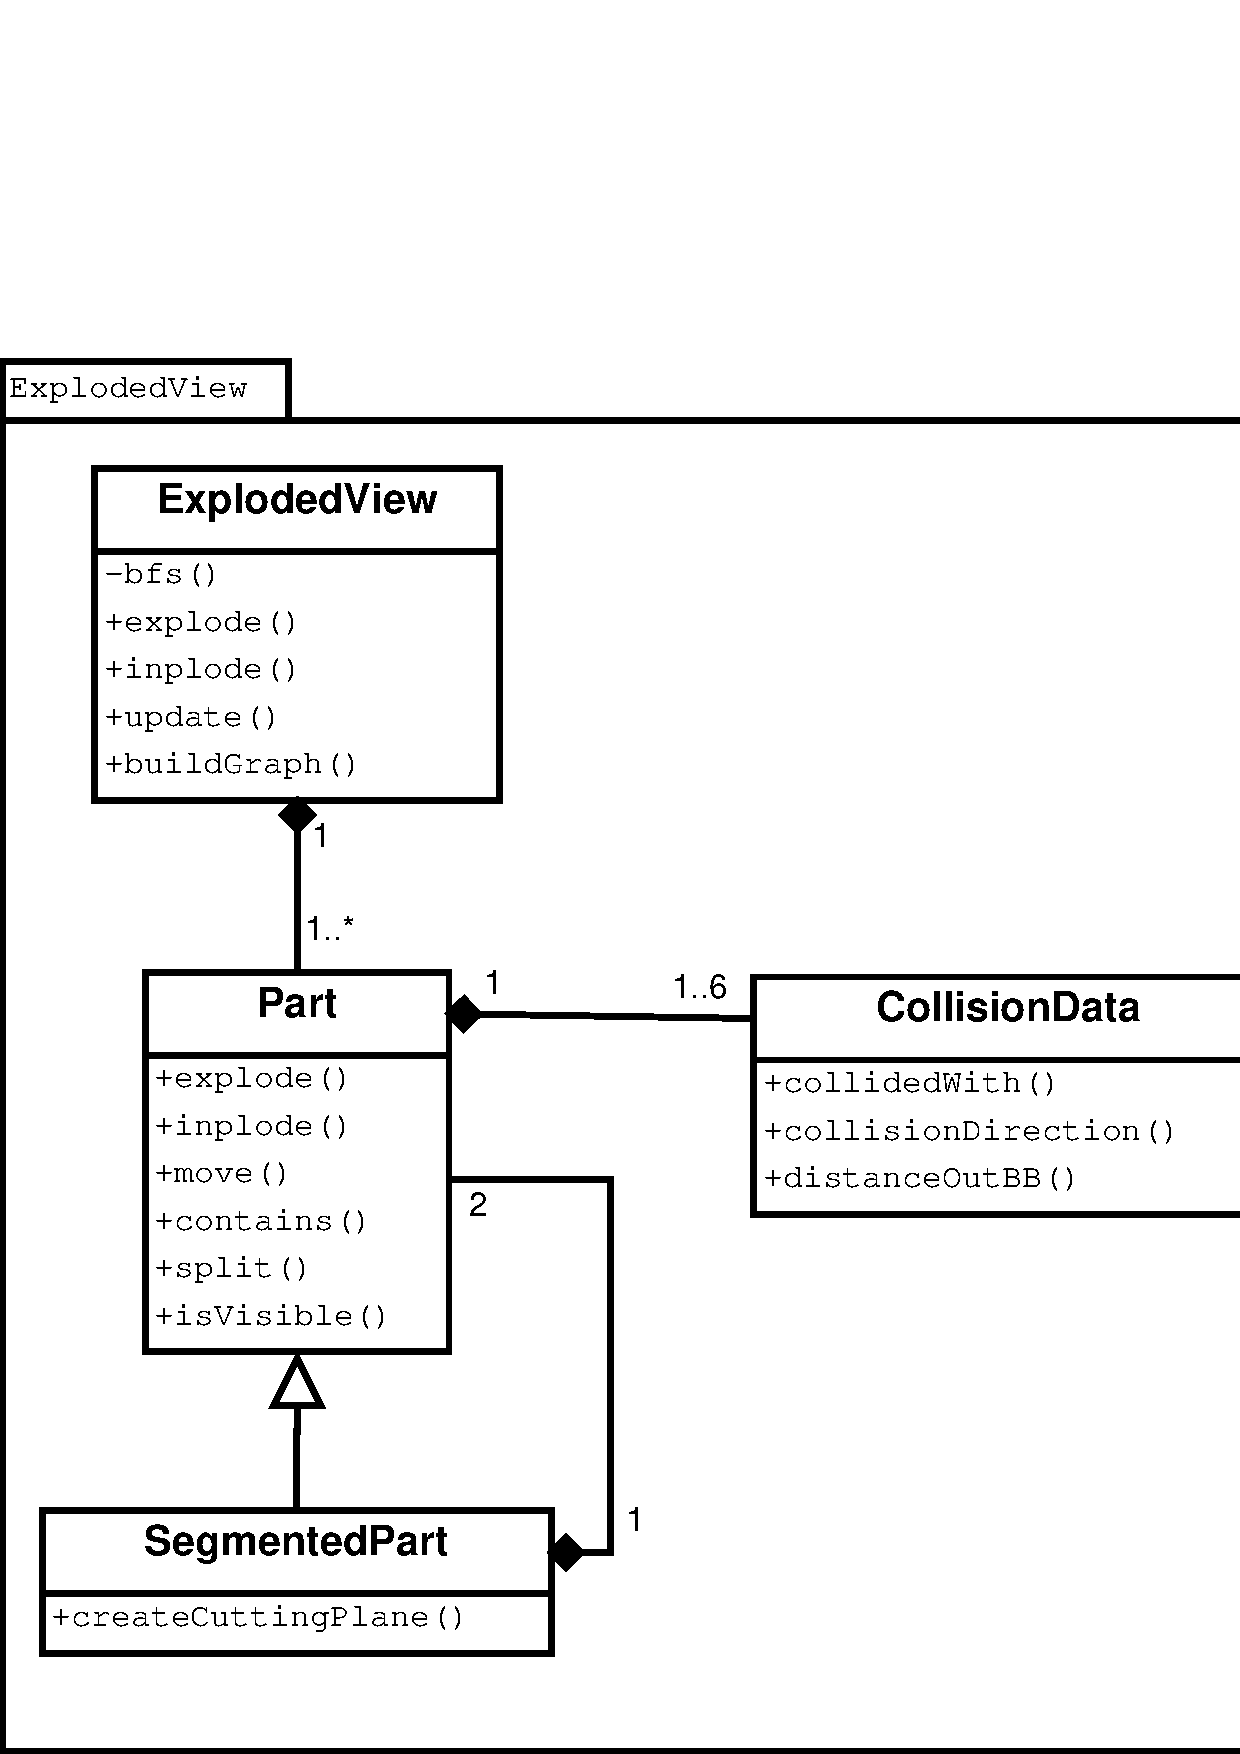
\includegraphics[height=0.8\linewidth]{img/arquitetura.pdf}}
	\caption[]{\label{fig:arquitetura} Vis�o geral da arquitetura}
\end{figure}

\begin{itemize}
	\item \textbf{ExplodedView}: classe geral, respons�vel pelo por tratar os dados de entrada (tanto o modelo 3D quanto o \emph{input} do usu�rio).
	\item \textbf{Part}textbf: classe que representa as partes do modelo.
	\item \textbf{SegmentedPart}: classe que herda de \textbf{Part} e representa os recipientes divididos.
	\item \textbf{CollisionData}: representa os dados de colis�o.
\end{itemize}

A gera��o do grafo de explos�o � feita logo no in�cio da execu��o do programa. As partes s�o extra�das do modelo 3D atrav�s de um \textbf{NodeVisitor} que procura pelos nomes dos n�s atrav�s de uma express�o regular. Cada n� (parte) � ent�o associado a um novo objeto do tipo \textbf{Part}.

Para a detec��o das dire��es obstru�das de cada parte, foi empregada duas abordagens. A primeira, explorada em \cite{882352}, constr�i um \emph{grafo de bloqueio direcional}

Considerando que o usu�rio quer explodir o n� $p$, o sistema implementado ir� executar uma busca em largura (\emph{BFS}) a partir de $p$ e armazenar o n�vel de cada n� descendente. A Figura \ref{fig:grafo} mostra os n�veis montados pela busca em largura para um modelo simples e a partir da parte $A$.

\begin{figure}[h]
	\center{\includegraphics[height=0.2\linewidth]{img/grafo.pdf}}
	\caption[]{\label{fig:grafo} Exemplo de n�veis da BFS}
\end{figure}

A explos�o e a implos�o do modelo ser� feita ent�o com base nessas n�veis, de forma simples:

\begin{algorithm}[H]
	\SetLine
	\Dados{$A_i$: n�veis de um grafo, $i < n$}
	\Para{$i = n..1$}{
		Explode n�s no n�vel $A_i$\;
	}
	\caption{Explos�o de uma parte}
	\label{alg:explosao}
\end{algorithm}

\begin{algorithm}[H]
	\SetLine
	\Dados{$A_i$: n�veis de um grafo, $i < n$}
	\Para{$i = 1..n$}{
		Implode n�s no n�vel $A_i$\;
	}
	\caption{Implos�o de uma parte}
	\label{alg:implosao}
\end{algorithm}


A divis�o dos recipientes (\emph{containers}) foi feita com o uso de um \textbf{ClipNode} do \textbf{OSG}, que ir� determinar o plano de corte para a parte ser renderizada.


\subsection{Caracter�sticas n�o abordadas}
Algumas caracter�sticas do sistema proposto em \cite{1360700} n�o foram implementadas, como ... .
\section{Resultados}

\begin{frame}\frametitle{V�deo}
V�deo (http://www.youtube.com/watch?v=31wx1-A9qZw)
\end{frame}

\begin{frame}\frametitle{Modelo 1}
\begin{figure}
	\center{\includegraphics[width=0.5\linewidth]{img/caps/test0_1.png}\includegraphics[width=0.5\linewidth]{img/caps/test0_2.png}}
\end{figure}
\end{frame}

\begin{frame}\frametitle{Modelo 2}
\begin{figure}
	\center{\includegraphics[width=0.3\linewidth]{img/caps/test1_1.png}\includegraphics[width=0.3\linewidth]{img/caps/test1_2.png}\includegraphics[width=0.3\linewidth]{img/caps/test1_3.png}}
\end{figure}
\end{frame}

\begin{frame}\frametitle{Modelo 3}
\begin{figure}
	\center{\includegraphics[width=0.5\linewidth]{img/caps/test2_1.png}\includegraphics[width=0.5\linewidth]{img/caps/test2_2.png}\\\includegraphics[width=0.5\linewidth]{img/caps/test2_3.png}\includegraphics[width=0.5\linewidth]{img/caps/test2_4.png}}
\end{figure}
\end{frame}

\begin{frame}\frametitle{Modelo 4}
\begin{figure}
	\center{\includegraphics[width=0.5\linewidth]{img/caps/test4_1.png}\includegraphics[width=0.5\linewidth]{img/caps/test4_2.png}\\\includegraphics[width=0.5\linewidth]{img/caps/test4_3.png}\includegraphics[width=0.5\linewidth]{img/caps/test4_4.png}}
\end{figure}
\end{frame}

\begin{frame}\frametitle{Modelo 5}
\begin{figure}
	\center{\includegraphics[width=0.5\linewidth]{img/caps/test9_1.png}\includegraphics[width=0.5\linewidth]{img/caps/test9_2.png}}
\end{figure}
\end{frame}

\begin{frame}\frametitle{Modelo 6}
\begin{figure}
	\center{\includegraphics[width=0.5\linewidth]{img/caps/test10_1.png}\includegraphics[width=0.5\linewidth]{img/caps/test10_2.png}}
\end{figure}
\end{frame}
\section{Conclus�o e Trabalhos Futuros}
Conclus�o e trabalhos futuros



%\section*{Acknowledgements}

%To Robert, for all the bagels.

\bibliographystyle{acmsiggraph}
%\nocite{*}
\bibliography{paper}


\newpage
\begin{figure*}
	\center{\includegraphics[width=0.5\linewidth]{img/caps/test0_1.png}\includegraphics[width=0.5\linewidth]{img/caps/test0_2.png}}
	\caption{\label{fig:test0} Modelo 1 antes e depois da explos�o da parte central.}
\end{figure*}

\begin{figure*}
	\center{\includegraphics[width=0.3\linewidth]{img/caps/test1_1.png}\includegraphics[width=0.3\linewidth]{img/caps/test1_2.png}\includegraphics[width=0.3\linewidth]{img/caps/test1_3.png}}
	\caption{\label{fig:test1} Modelo 2 antes e depois da explos�o da parte central, e alterando a posi��o da c�mera.}
\end{figure*}

\begin{figure*}
	\center{\includegraphics[width=0.5\linewidth]{img/caps/test2_1.png}\includegraphics[width=0.5\linewidth]{img/caps/test2_2.png}\\\includegraphics[width=0.5\linewidth]{img/caps/test2_3.png}\includegraphics[width=0.5\linewidth]{img/caps/test2_4.png}}
	\caption{\label{fig:test2} Modelo 3 antes e depois da explos�o da parte central, e alterando a posi��o da c�mera.}
\end{figure*}

\begin{figure*}
	\center{\includegraphics[width=0.5\linewidth]{img/caps/test4_1.png}\includegraphics[width=0.5\linewidth]{img/caps/test4_2.png}\\\includegraphics[width=0.5\linewidth]{img/caps/test4_3.png}\includegraphics[width=0.5\linewidth]{img/caps/test4_4.png}}
	\caption{\label{fig:test4} Modelo 4 antes e depois da explos�o da parte central, com uma parte envolvendo totalmente outra parte.}
\end{figure*}


\begin{figure*}
	\center{\includegraphics[width=0.5\linewidth]{img/caps/test9_1.png}\includegraphics[width=0.5\linewidth]{img/caps/test9_2.png}}
	\caption{\label{fig:test9} Modelo 5 antes e depois da explos�o da parte central.}
\end{figure*}

\begin{figure*}
	\center{\includegraphics[width=0.5\linewidth]{img/caps/test10_1.png}\includegraphics[width=0.5\linewidth]{img/caps/test10_2.png}}
	\caption{\label{fig:test10} Modelo 6 antes e depois da explos�o da parte central.}
\end{figure*}

\end{document}
